\documentclass[11pt,a4paper]{article}

\usepackage{amssymb,amsmath,amsfonts}    %ams
\usepackage{wasysym} %des symboles
\usepackage[tmargin=1in,bmargin=1in,lmargin=.75in,rmargin=.75in]{geometry}
\usepackage{graphicx}
\usepackage{verbatim}
\usepackage{enumerate}
\usepackage{tikz}
\usetikzlibrary{calc,positioning,backgrounds}

\usepackage[utf8]{inputenc} 
\usepackage{listings}

\newcommand{\R}{{\mathbb R}}   % reals
\newcommand{\Q}{{\mathbb Q}}   % rationals
\newcommand{\N}{{\mathbb N}}   %natural numbers
\newcommand{\Z}{{\mathbb Z}}    %integers
\renewcommand{\P}{{\mathbb P}}   %primes
\newcommand{\F}{{\mathbb F}}

\newcommand\cc{{\cal C}}
\newcommand{\cw}{{\cal W}}



\newtheorem{theorem}{Theorem}
\newtheorem{cor}{Corollary}
\newtheorem{example}{Example}
\newtheorem{lemma}{Lemma}
\newtheorem{newcommandi}{Definition}


\newcommand{\proof}{\noindent {\bf Proof.\ \ }}

\newcommand{\qed}{\hfill $\square$}


\newcommand{\card}[1]{\vert #1 \vert}

\usepackage{fancybox}
\usepackage[french]{babel}
\usepackage{multicol}
\setlength{\columnseprule}{0.2pt}
\setlength{\columnsep}{16pt}
\usepackage{fancyhdr} % personalisation tete/pied de page



% CODE C
\lstdefinelanguage{pseudoC}%
  {morekeywords={auto,break\c{c}ase\c{c}har\c{c}onst\c{c}ontinue,default,do,double,%
     else,enum,extern,float,for,goto,if,int,long,register,return,%
     short,signed,sizeof,static,struct,switch,typedef,union,unsigned,%
     void,volatile,while},%
     sensitive,%
     morecomment=[s]{/*}{*/},%
     morecomment=[l]//,% nonstandard
     morestring=[b]",%
     morestring=[m]',% changed from `b' to `m'
     moredelim=*[directive]\#,%
     moredirectives={define,elif,else,endif,error,if,ifdef,ifndef,line,%
     include,pragma,undef,warning}}[keywords,comments,strings,directives]%
     
\lstdefinestyle{pseudoc}{
     language=pseudoC,
     basicstyle=\ttfamily,
%      basicstyle=\small\sffamily,
%      numbers=left,
%      numberstyle=\tiny,
%      frame=L,
     columns=fullflexible,
     showstringspaces=false
     }

\lstnewenvironment{ccode}{
\lstset{style=pseudoc}}{}

\lhead{Initiation au développement: python et algorithmique}
\rhead{\thepage}
\cfoot{}
\addtolength{\headheight}{50pt}

\setlength{\parindent}{0pt}

\title{Initiation au développement: python et algorithmique}
\author{BUT Informatique\\
IUT de Vélizy\\
année 2021-2022}
\date{}

\catcode`\_=12 %for escaping underscore

\usepackage{marginnote}
\usepackage{fancyvrb} % Verbatim avancé

\newcommand{\reflexion}{\hspace{-1.2cm} 
\includegraphics[width=1cm]{img/reflexion.jpg} \vskip -.8cm}
%\newcommand{\checkbox}{
\includegraphics[width=.5cm]{checkbox.jpg} }
\newcommand{\checkbox}{$\square$ \smallskip}


%%environement pour le symbole lecture et un decalage
\newenvironment{lecture}{%
\smallskip
\begin{tabular}{c|c}
    \hspace{.03\textwidth} 
\includegraphics[width=.07\textwidth]{img/lecture.jpg} & 
\begin{minipage}{.85\textwidth}
}{%
\end{minipage}
\end{tabular}
}



\newcounter{exo} \setcounter{exo}{0}
\newenvironment{action}{%
    \begin{enumerate}[\numerotation] \addtocounter{exo}{-1}%
        }{%
    \end{enumerate}
}

%environement pour liste avec checkbox avec compteur
\newcommand{\numexoa}{\theexo \addtocounter{exo}{1}}
\newcommand{\numerotation}{\checkbox \smallskip \numexoa.}

%%environement de validation
\newenvironment{validation}{%
\smallskip
\begin{tabular}{c|c}
    \hspace{.03\textwidth} 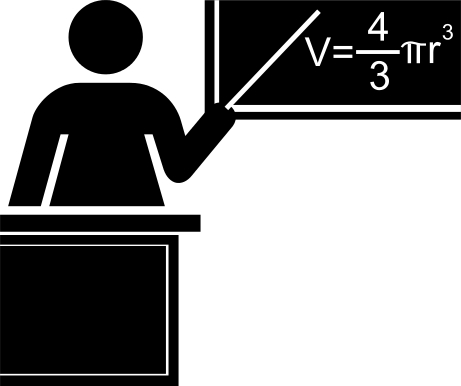
\includegraphics[width=.07\textwidth]{img/teacher.jpg} & 
\begin{minipage}{.85\textwidth}
}{%
\end{minipage}\\
\hline
\end{tabular}
}


%pour les fichiers c et dossiers
\newcounter{exoo} \setcounter{exoo}{0}
\newcommand{\numexo}{\theexoo}
\newcommand{\repexo}{{\tt exo_\numexo}}
\newcommand{\exoplus}{\addtocounter{exoo}{1}}




\begin{document}
% \maketitle





\thispagestyle{empty}


\newpage 
\hfill {\it (version 16/11/2021)}
\begin{center}
    \fcolorbox{gray!50}{gray!50}{\Large \tt Notice d'utilisation de la bibliothèque graphique {\tt tkiteasy}}
\end{center}

{\tt tkiteasy} est une librairie "{\it maison}" qui va vous permettre de gérer des graphismes sans avoir besoin de vous plonger dans les méandres techniques de {\tt tkinter}. Elle est en fait une interface simple entre vous et ce module {\tt tkinter} qui nécessite un certain apprentissage.

\section{Installation de la librairie {\tt tkiteasy}}
La librairie {\tt tkiteasy} est écrite en {\tt python3}. Elle s'appuie sur la librairie graphique {\tt tkinter}. Elle nécessite également la librairie {\tt PIL}, qui permet de gérer des images. Pour utiliser {\tt tkiteasy}, vous devez donc installer les paquets {\tt python3-tk}, {\tt python3-pil} et {\tt python3-pil.imagetk} .

\section{Ouverture de session graphique et objet Canevas}
La première méthode (c'est à dire fonction) à utiliser pour pouvoir lancer {\tt tkiteasy} est {\tt ouvrirFenetre(x,y)}, où {\tt x} indique la largeur en pixels de la fenêtre graphique, et où {\tt y} indique sa hauteur. Exemple de lancement d'une session graphique:
\begin{ccode}
    g = ouvrirFenetre(800,600)
\end{ccode}
On a ici créé une fenêtre de 800 pixels de large sur 600 pixels de haut.\\
{\bf IMPORTANT: le point de coordonnées {\tt (0,0)} se trouve toujours en haut à gauche de la fenêtre.}\\

L'appel à {\tt ouvrirFenetre} renvoie un objet {\tt Canevas} (ici {\tt g}). C'est un objet que vous devez conserver et utiliser tout au long de votre programme. Il vous permettra de lancer les méthodes graphiques qui sont présentées ci-dessous.

\section{Méthodes du {\tt Canevas}}
\`A partir du moment où vous disposez d'un {\tt Canevas}, vous allez pouvoir créez et manipuler toutes sortes de figures géométriques, textes, images dans votre fenêtre graphique. Voici les méthodes permettant de créer ces figures.\\
Le fichier {\tt main.py} fourni avec {\tt tkiteasy} vous montre comment manipuler ces objets graphiques et lancer les différentes méthodes de la librairie.

\subsection*{Création de figures géométriques, images, textes}

\subsubsection*{\fbox{\tt dessinerRectangle(x, y, l, h, col)}}
Crée un rectangle plein, dont le coin supérieur gauche se trouve en {\tt (x,y)}, dont la largeur est {\tt l}, la hauteur {\tt h} et la couleur {\tt col} (voir la \underline{section dédiée aux couleurs}).\\

{\bf IMPORTANT : cette méthode, ainsi que toutes les méthodes qui créent des figures géométriques, renvoie un objet. Vous pouvez récupérer cet objet dans une variable, ce qui vous permettra ensuite de le modifier, le déplacer, le supprimer, ou bien ignorer cet objet si vous pensez ne plus en avoir besoin ultérieurement.}

\subsubsection*{\fbox{\tt dessinerLigne(x, y, x2, y2, col)}}
Cette méthode dessine une ligne entre le point {\tt (x,y)} et le point {\tt (x2, y2)}, de couleur {\tt col}.

\subsubsection*{\fbox{\tt dessinerCercle(x, y, r, col)}}
Dessine un cercle de centre {\tt (x,y)} et de rayon {\tt r}, de couleur {\tt col}.

\subsubsection*{\fbox{\tt dessinerDisque(x, y, r, col)}}
Dessine un disque de centre {\tt (x,y)} et de rayon {\tt r}, de couleur {\tt col}.

\subsubsection*{\fbox{\tt changerPixel(x, y, col)}}
Dessine un pixel de coordonnées {\tt (x,y)} et de couleur {\tt col}.

\subsubsection*{\fbox{\tt afficherTexte(txt, x, y, col, sizefont)}}
\'Ecrit un texte {\tt txt} en position {\tt (x,y)}, de couleur {\tt col} (blanc par défaut) et de taille {\tt sizefont} (18 par défaut).

\subsubsection*{\fbox{\tt afficherImage(x, y, filename)}}
Affiche une image en position {\tt (x,y)}, provenant du fichier {\tt filename}. Le fichier doit être précisé {\bf avec son chemin relatif au script python}. Cette méthode accepte les principaux formats bruts ({\tt PNG, BMP}) ou compressés ({\tt JPG, GIF}).

\subsection*{Méthodes de modification d'objets existants}
Les méthodes qui suivent permettent de modifier un objet existant: changer ses caractéristiques (couleur, texte), le déplacer ou le supprimer. Pour ce faire, vous devez avoir conservé une référence à l'objet créé, au moment de sa création. Voir exemple ci-dessous.
\subsubsection*{\fbox{\tt deplacer(obj, dx, dy)}}
Permet de déplacer un objet {\tt obj} de {\tt dx} pixels horizontalement et {\tt dy} pixels verticalement.\\
Exemple:
\begin{ccode}
    c = g.dessinerCercle(800,600,10,"pink") # c contient une référence au cercle créé
    # plus tard dans le programme...
    g.deplacer(c, 10, 0) # ...on déplace le cercle de 10 pixels vers la droite en utilisant cette référence
\end{ccode}

\subsubsection*{\fbox{\tt supprimer(obj)}}
Supprime l'objet {\tt obj}.

\subsubsection*{\fbox{\tt changerCouleur(obj, col)}}
Change la couleur de l'objet {\tt obj} en {\tt col}.

\subsubsection*{\fbox{\tt changerTexte(obj, txt)}}
Change le texte de l'objet {\tt obj} (nécessairement un objet texte) en {\tt txt}.

\newpage
\subsection*{Gestion des événements}
On appelle {\it événement} une interaction entre l'utilisateur et le programme: clic souris, appui touche clavier, déplacement souris.

\subsubsection*{\fbox{\tt recupererTouche()}}
Permet de récupérer la dernière touche pressée au clavier. La variable renvoyée est une {\it string} qui contient la description de la touche: {\tt "a", "b", "c",}... Elle peut également contenir le nom de certaines touches spéciales (curseurs, touche de fonction...) : {\tt "Right", "Left", "Up", "Down",}...voir la \underline{section dédiée aux touches clavier}. La variable contient {\tt None} si aucune touche n'a été presséei depuis la dernière récupération de touche.

\subsubsection*{\fbox{\tt attendreTouche()}}
Même fonctionnement que la méthode précédente (renvoie la touche cliquée), mais la fonction est bloquante: elle bloque le programme et attend une touche.

\subsubsection*{\fbox{\tt recupererClic()}}
Permet de récupérer la position du dernier clic gauche de souris. La variable renvoyée est un {\tt Event} qui contient des champs {\tt x} et {\tt y}. Ainsi, vous pouvez obtenir les coordonnées du point cliqué de la façon suivante:
\begin{ccode}
    p = g.recupererClic()
    print(p.x, p.y)
\end{ccode}
Si aucun clic n'a eu lieu depuis la dernière récupération de position, la méthode renvoie {\tt None}. Un champ {\tt num} permet également de tester quel bouton a été cliqué: {\tt num=1} pour le bouton gauche, {\tt num=3} pour le bouton droit.

\subsubsection*{\fbox{\tt attendreClic()}}
Même fonctionnement que la méthode précédente (renvoie la position cliquée), mais la fonction est bloquante: elle bloque le programme et attend le clic.

\subsubsection*{\fbox{\tt recupererPosition()}}
Permet de récupérer la dernière position de souris suite à un déplacement de souris. La variable renvoyée est un {\tt Event} qui contient des champs {\tt x} et {\tt y}: les coordonnées {\tt (x,y)} de la souris, ou {\tt (0,0)} si aucun déplacement n'a eu lieu depuis le lancement du programme.


\subsection*{Autres fonctions}

\subsubsection*{\fbox{\tt actualiser()}}
Cette méothode, placée après une méthode graphique, force le rafraîchissment. \`A utiliser avec modération au risque de ralentir votre programme.\\

{\bf IMPORTANT}: Lorsqu'on crée ou qu'on modifie un objet graphique, il n'est pas modifié immédiatement à l'écran. Le système de gestion graphique attend un certain temps pour effectuer ce rafraîchissement, afin de réunir plusieurs modifications et réduire ainsi le nombre de rafraîchissements, opérations assez coûteuses.\\
Si vous dessinez un simple objet graphique, vous n'aurez donc pas besoin de forcer un rafraîchissement de l'écran. Mais lorsqu'on demande de nombreuses modifications, comme par exemple lorsqu'on déplace de nombreux objets simultanément, cela peut devenir nécessaire.\\
{\bf Si vous ne voyez pas à l'écran les résultats des fonctions graphiques que vous avez appelées, essayez un {\tt actualiser()}!}

\subsubsection*{\fbox{\tt pause(sec)}}
Parfois, le programme crée se déroule trop rapidement et nécessite d'être ralenti. Cette méthode permet de forcer une pause, d'une durée de {\tt sec} secondes. {\tt sec} est un flottant, on peut donc demander une pause en dixièmes, centièmes, millièmes de secondes. Par défaut, cette méthode crée une pause d'une demi milliseconde.

\subsubsection*{\fbox{\tt fermerFenetre()}}
Ferme la fenêtre graphique.

\section{{\tt ObjetGraphique}}
Toutes les méthodes qui créent des objets graphiques (rectangle, disque, image...etc) renvoient un {\tt ObjetGraphique}. Cet {\tt ObjetGraphique} contient trois champs utiles si vous souhaitez récupérer certaines informations concernant cet objet:
\begin{itemize}
  \item {\tt x} et {\tt y}, qui contiennent les coordonnées actuelles de l'objet
  \item {\tt col}, qui contient sa couleur
\end{itemize}

\section{Les couleurs}
Il existe deux façons d'indiquer une couleur:
\begin{itemize}
  \item par son code RVB sous la forme hexadécimale: {\tt \#rrvvbb} où {\tt rr,vv,bb} sont les composantes rouges, vertes et bleues de la couleur souhaitée. Exemple: {\tt \#ff0000} indique le rouge.\\ 
  {\bf ATTENTION}: cet hexadécimal doit être transmis sous forme de {\tt string}.\\
  Exemple: {\tt dessinerCercle(x,y,r,"#ff00ab")}
  \item par une {\tt string} prédéfinie. Les couleurs {\tt 'white', 'black', 'red', 'green', 'blue', 'cyan', 'yellow'}, et {\tt 'magenta'} sont toujours disponibles. De nombreuses autres couleurs le sont également, en fonction de la configuration locale de votre ordinateur. Faites des tentatives: {\tt "pink", "gold",}...
\end{itemize}

\section{Les touches clavier}
\begin{tabular}{ll}
{\tt Return} 	& 	La touche Entrée\\
{\tt space} 	& 	La barre espace\\
{\tt Tab} 	& 	La touche de Tabulation, Tab\\

{\tt Up} 	& 	↑\\
{\tt Down} 	& 	↓\\
{\tt Left} 	& 	←\\
{\tt Right} 	& 	→\\
&\\
{\tt Alt\_L} 	& 	La touche Alt située à gauche.\\
{\tt Alt\_R} 	& 	La touche Alt située à droite.\\
{\tt Control\_L} 	& 	La touche Ctrl de gauche\\
{\tt Control\_R} 	& 	La touche Ctrl de droite\\
{\tt Shift\_L} 	& 	La touche Maj de gauche\\
{\tt Shift\_R} 	& 	La touche Maj de droite\\
{\tt Caps\_Lock} 	& 	Verr Maj\\
{\tt Delete} 	& 	Suppr\\
{\tt BackSpace} 	& 	La touche Retour Arrière\\
{\tt Home} 	& 	Début\\
{\tt End} 	& 	Fin\\
{\tt Insert} 	& 	Inser\\
{\tt Escape} 	& 	Echap\\
{\tt F1} 	& 	La touche fonction F1\\
{\tt F2} 	& 	La touche fonction F2\\
{\tt Next} 	& 	PageDown\\
{\tt Prior} 	& 	PageUp\\
{\tt Pause} 	& 	Pause\\
{\tt Num\_Lock} 	& 	Verr Num\\
{\tt Print} 	& 	ImprÉcran\\
&\\
{\tt KP\_0} 	& 	0 sur le clavier numérique\\
{\tt KP\_1} 	& 	1 sur le clavier numérique\\
{\tt KP\_Up} 	& 	↑ sur le clavier numérique\\
{\tt KP\_Down} 	& 	↓ sur le clavier numérique\\
{\tt KP\_Left} 	& 	← sur le clavier numérique\\
{\tt KP\_Right} 	& 	→ sur le clavier numérique\\
{\tt KP\_Add} 	& 	+ sur le clavier numérique\\
{\tt KP\_Multiply} 	& 	× sur le clavier numérique\\
{\tt KP\_Subtract} 	& 	- sur le clavier numérique\\
{\tt KP\_Divide} 	& 	/ sur le clavier numérique\\
{\tt KP\_Next} 	& 	PageDown sur le clavier numérique\\
{\tt KP\_Prior} 	& 	PageUp sur le clavier numérique\\
{\tt KP\_Decimal} 	& 	Symbole de la ponctuation décimale (,) sur le clavier numérique\\
{\tt KP\_Delete} 	& 	Suppr sur le clavier numérique\\
{\tt KP\_End} 	& 	Fin sur le clavier numérique\\
{\tt KP\_Enter} 	& 	Entrée sur le clavier numérique\\
{\tt KP\_Home} 	& 	Début sur le clavier numérique\\
{\tt KP\_Insert} 	& 	Insert sur le clavier numérique\\
\end{tabular}{}

\end{document}
